% ============================================================================
%  Master's thesis -- OpenSearch@DLR 2.0, Work Package 2, Milestone 2.1
%
%  Unsupervised Discovery of Fine-Grained Topics in Web Corpora
%
%  Compile:  tectonic -X compile main.tex
%       or:  pdflatex main.tex  (twice, for the table of contents)
%  Standard packages only -- compiles as-is on Overleaf.
% ============================================================================
\documentclass[11pt,a4paper]{article}

\usepackage[T1]{fontenc}
\usepackage[utf8]{inputenc}
\usepackage[a4paper,margin=2.4cm]{geometry}
\usepackage{amssymb,amsmath}
\usepackage{booktabs}
\usepackage{array}
\usepackage{xcolor}
\usepackage{enumitem}
\usepackage{caption}
\usepackage{microtype}
\usepackage{longtable}
\usepackage{graphicx}
\usepackage{tikz}
\usetikzlibrary{arrows.meta,positioning,calc}
\usepackage[hidelinks]{hyperref}

% --- colours ----------------------------------------------------------------
\definecolor{accent}{HTML}{12556A}
\definecolor{good}{HTML}{2C6E49}
\definecolor{bad}{HTML}{A33A3A}
% diagram palette (Figure 1)
\definecolor{boxblue}{HTML}{3D7DD8}
\definecolor{fillblue}{HTML}{E3EDFB}
\definecolor{boxgreen}{HTML}{1E9E63}
\definecolor{fillgreen}{HTML}{E4F4EB}
\definecolor{boxred}{HTML}{E2553A}
\definecolor{fillred}{HTML}{FBE9E3}
\definecolor{diagray}{HTML}{8A8A8A}
\hypersetup{colorlinks=true,linkcolor=accent,urlcolor=accent,citecolor=accent}

% --- spacing ----------------------------------------------------------------
\setlength{\parindent}{0pt}
\setlength{\parskip}{0.55em}
\captionsetup{font=small,labelfont=bf,labelsep=period}
\renewcommand{\arraystretch}{1.15}

% --- semantic commands ------------------------------------------------------
% held / positive results and failed / retracted ones, marked consistently
\newcommand{\gd}[1]{\textcolor{good}{\textbf{#1}}}
\newcommand{\bd}[1]{\textcolor{bad}{\textbf{#1}}}
% claim register: what kind of evidence stands behind a statement
\newcommand{\proved}{\textcolor{accent}{\textsf{\footnotesize[proved]}}}
\newcommand{\measured}{\textcolor{accent}{\textsf{\footnotesize[measured]}}}
\newcommand{\tg}[1]{{\footnotesize\textsf{[#1]}}}

\begin{document}

% ---------------------------------------------------------------- TITLE PAGE
\begin{titlepage}
\centering
\vspace*{1.8cm}

{\footnotesize\sffamily\textcolor{accent}%
{OPENSEARCH@DLR 2.0 \quad$\cdot$\quad WORK PACKAGE 2 \quad$\cdot$\quad MILESTONE 2.1}}\\[0.35cm]
{\footnotesize\sffamily\textcolor{accent}{MASTER'S THESIS}}\\[1.5cm]

{\LARGE\bfseries Unsupervised Discovery of\\[0.25cm]
Fine-Grained Topics in Web Corpora\par}
\vfill
\end{titlepage}


% Working outline: old prose cleared on 2026-11-09.
\section*{Abstract}
\addcontentsline{toc}{section}{Abstract}



{\hypersetup{linkcolor=black}\tableofcontents}
\clearpage

% Working outline: old prose cleared on 2026-11-09.
\section{Introduction}

\subsection{The problem}

\subsection{Constraints}
\label{sec:intro-neutrality}

\subsection{Research questions}

\subsection{Contributions}

\subsection{A note on how claims are marked}


% Working outline: old prose cleared on 2026-11-09.
\section{Related work and positioning}
\label{sec:related}

\subsection{Topic models}

\subsection{Embeddings}

\subsection{Hierarchical topic models, and why they do not answer RQ3}

\subsection{Matching topics across models}

\subsection{The novelty claim, stated narrowly}

\subsection{Evaluating topic models without an answer key}


% --------------------------------------------------------------------- METHOD
\section{Data and method}
\label{sec:method}

\subsection{The motivating corpus}
\label{sec:method-corpus}

The corpus is a crawl of a large research organisation's public websites, collected for this
project between 21 March and 11 October 2022 across 80 hosts~\cite{dlrcrawl2022}. It is not a published
dataset: it is not redistributable and cannot be obtained by a reader. That is a
real limitation on reproducibility, and it is why Section~\ref{sec:neutrality} provides an
indirect check using three corpora that anyone can download.
\measured{} The raw crawl spans 45 detected languages, but English and German account for
89.7\% of it, and only those two are carried forward. The corpus's role here is to supply
realistic scale and realistic mess; the method is not specialised to it.

\begin{samepage}
\measured{} The original crawl contains 733{,}210 archived records. After language selection
and text cleaning, the final corpus used for production labelling contains 616{,}499 records:
423{,}966 English and 192{,}533 German. Each record represents an archived capture of a page.
Distinct records can therefore share the same URL or contain identical text.
\end{samepage}

\begin{table}[h]\centering
\caption{Number of records in the original crawl and the final corpus used for production
labelling.}
\label{tab:corpus}
\begin{tabular}{lr}
\toprule
Stage & Records \\
\midrule
Original crawl                  & 733{,}210 \\
Final English--German corpus    & \gd{616{,}499} \\
\bottomrule
\end{tabular}
\end{table}

Production labelling uses the final 616{,}499-record corpus. Some earlier topic-model results
were retained without rerunning them after duplicate embedding rows were removed, as documented
in Section~\ref{sec:failures}.

\begin{figure}[t]\centering
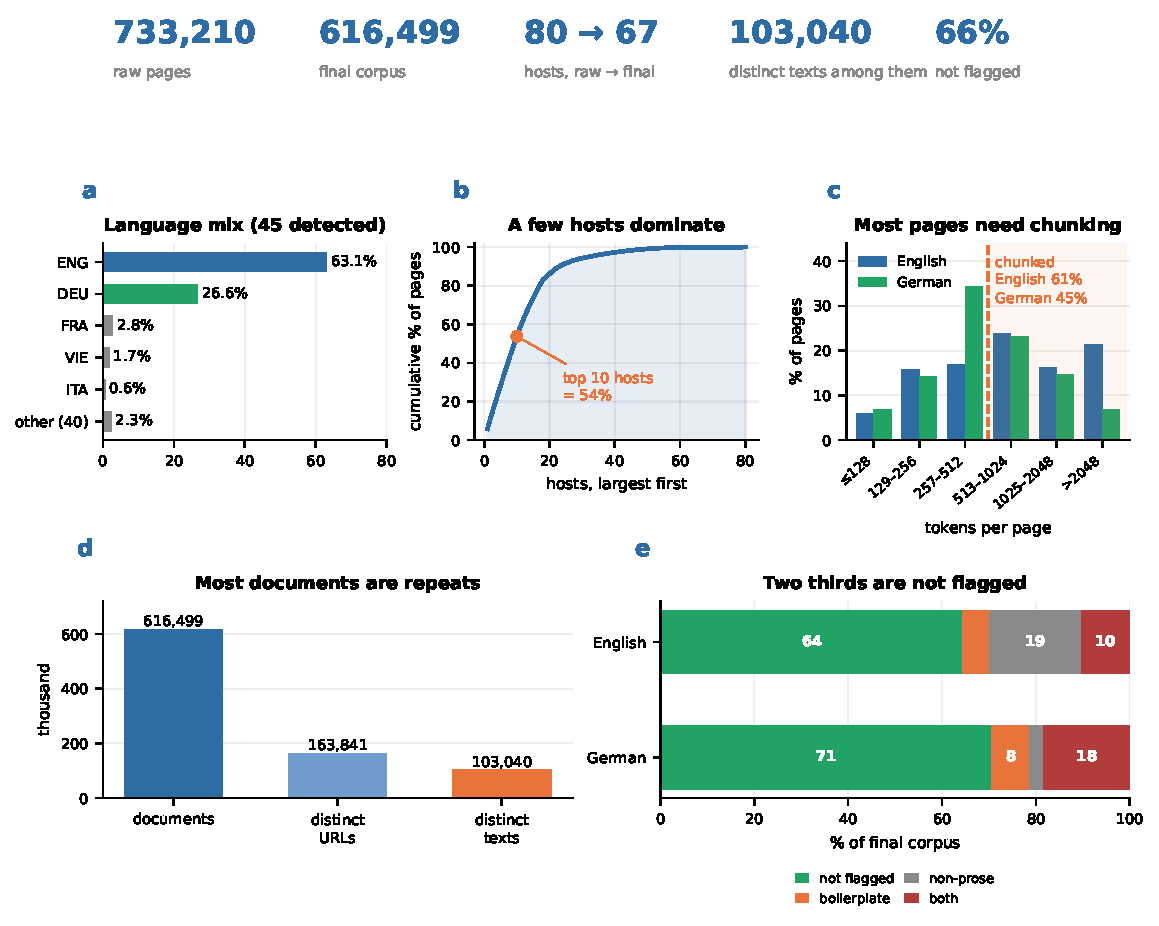
\includegraphics[width=\textwidth]{figs/fig_crawl_dashboard}
\caption{Profile of the DLR crawl. The strip gives the headline counts.
\textbf{(a)}~Detected languages in the raw crawl; records without a detected language are not
shown. Only English and German are modelled.
\textbf{(b)}~Cumulative share of pages held by the largest hosts, where a host is a subdomain of
\texttt{dlr.de}.
\textbf{(c)}~Share of pages in the final corpus in each length band, in tokens, against the 512-token
window of the embedding model; pages right of the dashed line must be split into chunks.
\textbf{(d)}~The 616{,}499 documents in the final corpus correspond to only 163{,}841 distinct URLs and
103{,}040 distinct texts, because the same page was fetched repeatedly.
\textbf{(e)}~Share of pages in the final corpus by the pipeline's boilerplate and non-prose flags.}
\label{fig:dashboard}
\end{figure}

\measured{} Figure~\ref{fig:dashboard} profiles the crawl. In the raw crawl English is 63.1\% of pages (462{,}595) and German 26.6\%
(195{,}133). A further 54{,}309 pages are in 43 other detected languages, and 21{,}173 have no
detected language. Among the other detected languages, French is the largest at 2.8\% of the raw
crawl, followed by Vietnamese at 1.7\% (Figure~\ref{fig:dashboard}a). Ten hosts hold 53.7\% of the raw
crawl and the largest alone 5.9\%, so the corpus is dominated by a few large sites
(Figure~\ref{fig:dashboard}b).

Two properties of the data drive design decisions later on. First, the same page is fetched
repeatedly: the final corpus holds 616{,}499 documents but only 163{,}841 distinct URLs
(3.8 per address) and only 103{,}040 distinct texts (6.0 documents per text;
Figure~\ref{fig:dashboard}d). The duplicate-removal step removes repeated copies of the same
record. Different captures with the same URL or text remain, so user-facing results must also
be de-duplicated by normalised address. Second, \measured{} the pipeline's detectors flag 33.6\%
of pages in the final corpus as boilerplate, non-prose or both. These flags target material such
as navigation, staff directories, search interfaces, privacy notices and machine-generated
artefacts. The flags were not checked page by page (Figure~\ref{fig:dashboard}e).

\subsection{The control and benchmark corpora}
\label{sec:method-benchmarks}

The crawl has no labels, so correctness cannot be measured on it directly. Four additional
corpora are used: one control for RQ1 and three labelled benchmarks for an indirect test of RQ3.
Topic models are fitted separately on each corpus. The corpora are deliberately unlike the crawl,
because transfer to dissimilar data is what the data-neutrality constraint of Section~\ref{sec:intro-neutrality}
requires in practice. Table~\ref{tab:datasets} lists them and Figure~\ref{fig:benchdash}
profiles them.

\begin{table}[h]\centering
\caption{The corpora used. Class shares are those of the largest and smallest class; the
largest is also the purity obtained by assigning every document to one cluster
(Section~\ref{sec:neutrality}). The control corpus carries no class labels in this work.}
\label{tab:datasets}
\small
\begin{tabular}{llrrrrr}
\toprule
Corpus & Language & Documents & Classes & Largest & Smallest & Median words \\
\midrule
DLR crawl (this work)~\cite{dlrcrawl2022}
                        & EN, DE & 616{,}499 & none & --- & --- & 310 \\
GDELT Ahrtal (control)~\cite{leetaru2013gdelt}
                        & DE     & 3{,}873 & none & --- & --- & 710 \\
\addlinespace
20 Newsgroups~\cite{lang1995newsweeder}
                        & EN     & 17{,}792 & 20 & 5.4\%  & 3.3\% & 89 \\
Reuters-21578~\cite{lewis1997reuters}
                        & EN     & 7{,}980  & 10 & 48.9\% & 1.4\% & 72 \\
10kGNAD~\cite{block2019gnad}
                        & DE     & 10{,}265 & 9  & 16.3\% & 5.2\% & 298 \\
\bottomrule
\end{tabular}
\end{table}

\begin{figure}[t]\centering
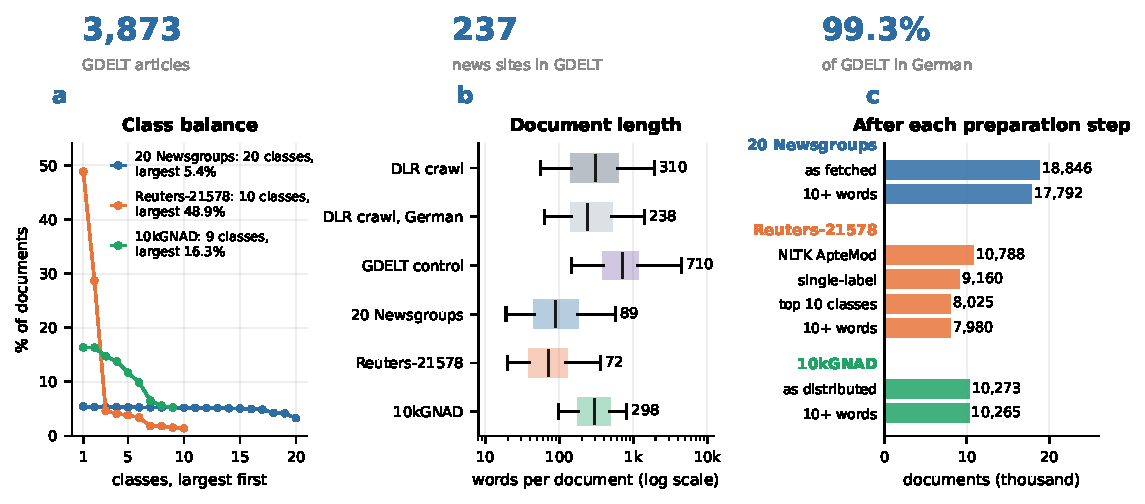
\includegraphics[width=\textwidth]{figs/fig_benchmark_dashboard}
\caption{Profile of the control and benchmark corpora. The strip gives the headline counts.
\textbf{(a)}~Share of documents in each class, largest class first, for the three labelled
benchmarks.
\textbf{(b)}~Words per document. Each box spans the middle half of the documents, the whiskers
the 5th to 95th percentile, and the number is the median.
\textbf{(c)}~Documents left after each preparation step.}
\label{fig:benchdash}
\end{figure}

\begin{samepage}
\paragraph{Preparation.} Documents under ten words are dropped from all three benchmarks.

20 Newsgroups has its headers, footers and quoted text removed, the
standard step that stops a model learning email boilerplate in place of
topics~\cite{sklearn20ng}. After this preparation and the minimum-length filter, 17{,}792 of
18{,}846 documents remain.
\end{samepage}

Reuters-21578 is taken from the ApteMod version distributed with NLTK (10{,}788 documents).
Only documents with one label are kept. Of these, only the ten most frequent categories are
retained, giving 8{,}025 documents. The minimum-length filter leaves 7{,}980.

10kGNAD, derived from the \emph{Der Standard} articles of the One Million Posts
corpus~\cite{schabus2017million}, is used as distributed. The minimum-length filter reduces
it from 10{,}273 to 10{,}265 documents (Figure~\ref{fig:benchdash}c).

\paragraph{Why these three.} 20 Newsgroups and Reuters-21578 are both English-only, which would
leave the German half of the pipeline with no external check, although German is a third of the
corpus (31.2\%). 10kGNAD was added to close that gap; its median length (298 words) is close to
the German crawl's (238). 20 Newsgroups has classes of nearly equal size, whereas almost half of
Reuters is one class (Figure~\ref{fig:benchdash}a). This matters when interpreting purity; Section~\ref{sec:experimental-purity-floor}
explains its lower bound.

\paragraph{The control corpus.} The GDELT control is a collection of 3{,}873 news articles about
a single event, the July 2021 flood in the Ahr valley, selected through GDELT's Global Knowledge
Graph~\cite{leetaru2013gdelt}. The articles come from 237 news sites and have GDELT-recorded dates
between July 2021 and August 2024, more than half of them in July 2021; 99.3\% are in German. It carries
no class labels. We use this corpus to check whether the difficulty comes from the
topic-discovery methods, the noisy DLR crawl, or both. GDELT covers the flood and the response
to it, so we expect a small number of topics. If a method still selects many topics here, this
points to a limitation of the method. If it selects only a few on GDELT but many on DLR, this
suggests that the DLR data explains the difference (Section~\ref{sec:rq1-nok}).

\measured{} The silhouette sweep in Figure~\ref{fig:gdelt-silhouette} supports this expectation. It tests different group counts
and compares how closely documents group together and how separate the groups are. On the
3{,}842 prepared articles, its highest score is 0.798 at $K=2$, meaning two groups, among the
tested values $K=2,4,\ldots,40$.\footnote{\raggedright The sweep uses Ward clustering on vectors
reduced to 50 coordinates with UMAP, scored by cosine silhouette. Saved configuration and
scores: \texttt{output/gdelt\_ahrtal/}\allowbreak\texttt{discover\_k/}, files
\texttt{k\_config.json} and \texttt{discover\_k\_silhouette.json}.}

\noindent\begin{minipage}{\linewidth}
\centering
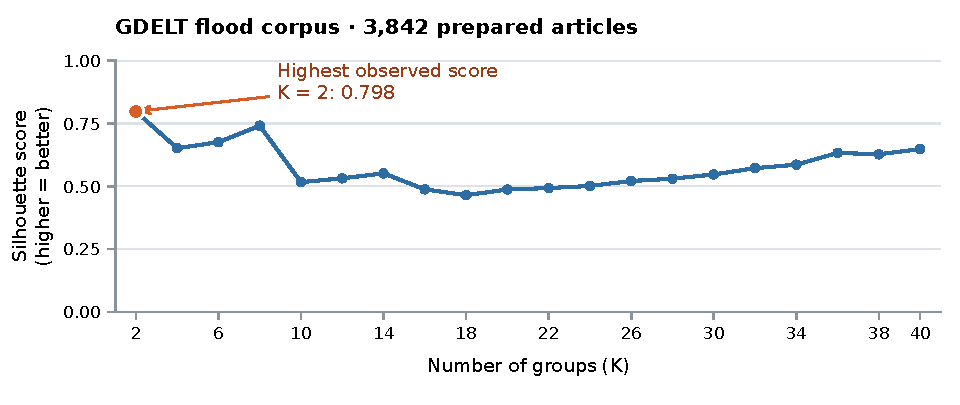
\includegraphics[width=\linewidth]{figs/fig_gdelt_silhouette.pdf}
\captionof{figure}{Silhouette sweep on the GDELT control. \measured{} Each dot is a tested
group count; lines connect the saved scores. The highlighted maximum occurs at the smallest
tested count. The prepared articles and scoring method are described above.}
\label{fig:gdelt-silhouette}
\end{minipage}

\paragraph{What the statistics drive.} \measured{} In the final corpus, the median page is 310
words and a quarter are under 148. The 5th to 95th percentile runs from 55 to 1{,}934 words, and
3.8\% of pages are under 50 words (Figure~\ref{fig:benchdash}b). Pages that short are hard to place.

Long pages raise a different problem. After text cleaning, 52.9\% of pages require more than one
chunk: 57.2\% in English and 43.4\% in German. Each chunk accommodates 494 text tokens, as
explained in Section~\ref{sec:method-embed}.

For comparison, a sample of 60{,}000 pages from the raw crawl has a median of 299 words, with
10\% of pages under 50 words. The final corpus contains a smaller share of very short pages.
This comparison combines language selection, minimum-length filtering and text cleaning.

The benchmark comparison has a separate implication. The two English benchmarks are far shorter
than the crawl, while 10kGNAD has a similar median length (Table~\ref{tab:datasets} and
Figure~\ref{fig:benchdash}b). These curated discussion and news collections differ from a
heterogeneous website crawl. They therefore provide a limited test of how the method handles
navigation pages, directories and other page types (Section~\ref{sec:limitations}).

\subsection{Pipeline}
\label{sec:method-pipeline}

The pipeline uses each page's cleaned body text as input. RQ2 (Section~\ref{sec:rq2}) explains
why body text was chosen.

Figure~\ref{fig:pipeline} summarises the production pipeline. The following subsections explain
embedding, topic discovery and document labeling in that order. The separate analyses used to
answer RQ3 are described in Section~\ref{sec:rq3}.

% ---------------------------------------------------------- PIPELINE FIGURE
\begin{figure}[!tb]
\centering
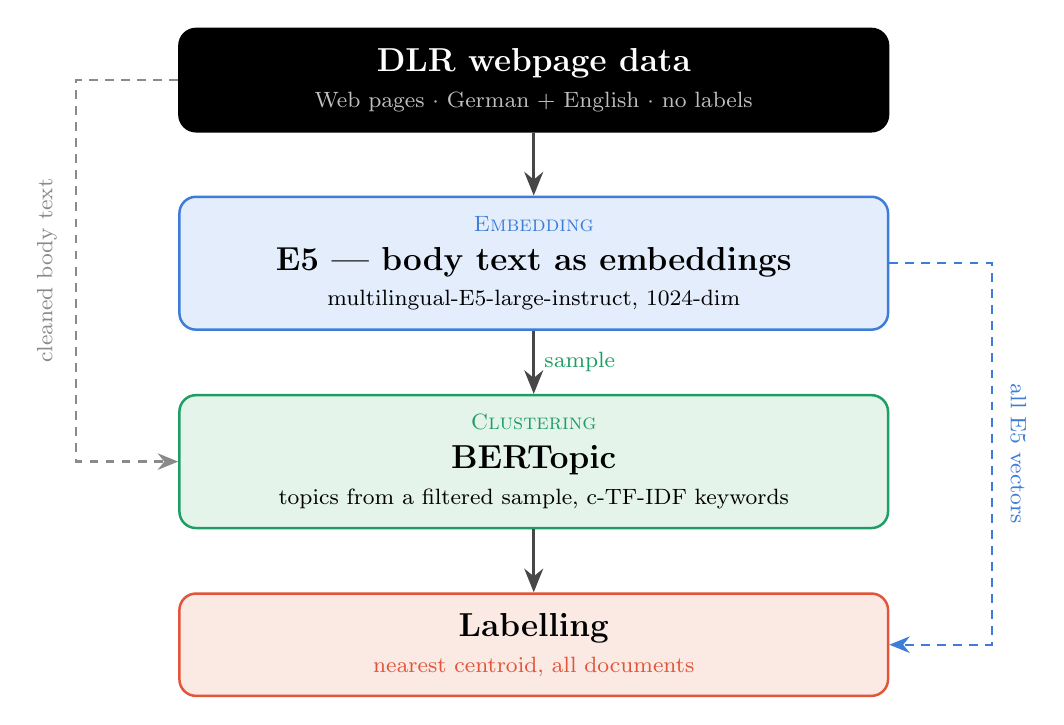
\begin{tikzpicture}[
  box/.style   = {rounded corners=6pt, draw, line width=0.9pt, minimum width=9.0cm,
                  minimum height=1.30cm, align=center, inner sep=7pt},
  flow/.style  = {-{Stealth[length=3mm,width=2.4mm]}, line width=1.1pt, draw=black!72},
  feed/.style  = {-{Stealth[length=2.6mm,width=2.1mm]}, line width=0.8pt, dashed,
                  dash pattern=on 3.2pt off 2.6pt},
]

% ---- nodes -----------------------------------------------------------------
\node[box, fill=black, draw=black, text=white] (data) at (0,0)
  {{\large\bfseries DLR webpage data}\\[1pt]
   {\footnotesize\color{black!25} Web pages $\cdot$ German $+$ English $\cdot$ no labels}};

\node[box, fill=fillblue, draw=boxblue, below=0.80cm of data] (embed)
  {{\footnotesize\scshape\color{boxblue} Embedding}\\[2pt]
   {\large\bfseries E5 --- body text as embeddings}\\[1pt]
   {\footnotesize multilingual-E5-large-instruct, 1024-dim}};

\node[box, fill=fillgreen, draw=boxgreen, below=0.80cm of embed] (cluster)
  {{\footnotesize\scshape\color{boxgreen} Clustering}\\[2pt]
   {\large\bfseries BERTopic}\\[1pt]
   {\footnotesize topics from a filtered sample, c-TF-IDF keywords}};

\node[box, fill=fillred, draw=boxred, below=0.80cm of cluster] (label)
  {{\large\bfseries Labelling}\\[1pt]
   {\footnotesize\color{boxred} nearest centroid, all documents}};

% ---- main flow -------------------------------------------------------------
\draw[flow] (data)    -- (embed);
\draw[flow] (embed)   -- node[right, font=\footnotesize, text=boxgreen] {sample} (cluster);
\draw[flow] (cluster) -- (label);

% ---- side feed: cleaned body text bypasses the embedder ------------------
\coordinate (lrail) at ($(data.west)+(-1.30,0)$);
\draw[feed, draw=diagray] (data.west) -- (lrail) |- (cluster.west);
\node[rotate=90, font=\footnotesize\color{diagray}, anchor=south]
  at ($(lrail)!0.5!(lrail|-cluster.west)+(-0.12,0)$) {cleaned body text};

% ---- side feed: E5 vectors reused for assignment ---------------------------
\coordinate (rrail) at ($(embed.east)+(1.30,0)$);
\draw[feed, draw=boxblue] (embed.east) -- (rrail) |- (label.east);
\node[rotate=-90, font=\footnotesize\color{boxblue}, anchor=south]
  at ($(rrail)!0.5!(rrail|-label.east)+(0.12,0)$) {all E5 vectors};

\end{tikzpicture}
\caption{The core document-assignment pipeline. E5 embeds all documents; BERTopic learns topics
from a filtered sample per language. The dashed paths supply cleaned body text for keywords
and all E5 vectors for nearest-centroid assignment. Every document receives a topic, including
those outside the sample.}
\label{fig:pipeline}
\end{figure}


\subsection{Document embeddings with E5}
\label{sec:method-embed}

The embedding model is \texttt{intfloat/}\allowbreak\texttt{multilingual-e5-large-instruct}
\cite{wang2024multilingual}. It converts each document's cleaned body text into a vector: a
list of 1{,}024 numbers representing the text. English and German use the same model. A fixed
task instruction asks it to identify the page's main research topic. The resulting vectors are
reused for topic discovery and document labeling.

E5 accepts 512 tokens, where a token is a word or part of a word. \measured{} In the
text before cleaning, the median page uses 1.84 tokens per word, so the window holds roughly 280
words; 56.1\% of pages are longer (Figure~\ref{fig:dashboard}c);
cutting those at 512 tokens would discard on average 54.8\% of their text. An attempt to raise the
window to 1{,}024 tokens failed because the model does not support that input length.

The fix adopted instead is to split each document into chunks that fit the window, embed
each chunk, and average the resulting vectors. Each chunk must also hold the model's 16-token task
instruction and two special tokens, which leaves 494 tokens of text, and the production embedding run keeps
at most eight chunks per document: its first 3{,}952 tokens.

Figure~\ref{fig:embedding-chunks} shows how pages are split into chunks and how much text the
eight-chunk limit leaves unread.
\measured{} On pages with text beyond this limit, an average of 51.4\% of their cleaned text
is left unread.
Most pages are read in full; the longest are represented by their beginning.

\noindent\begin{minipage}{\linewidth}
\centering
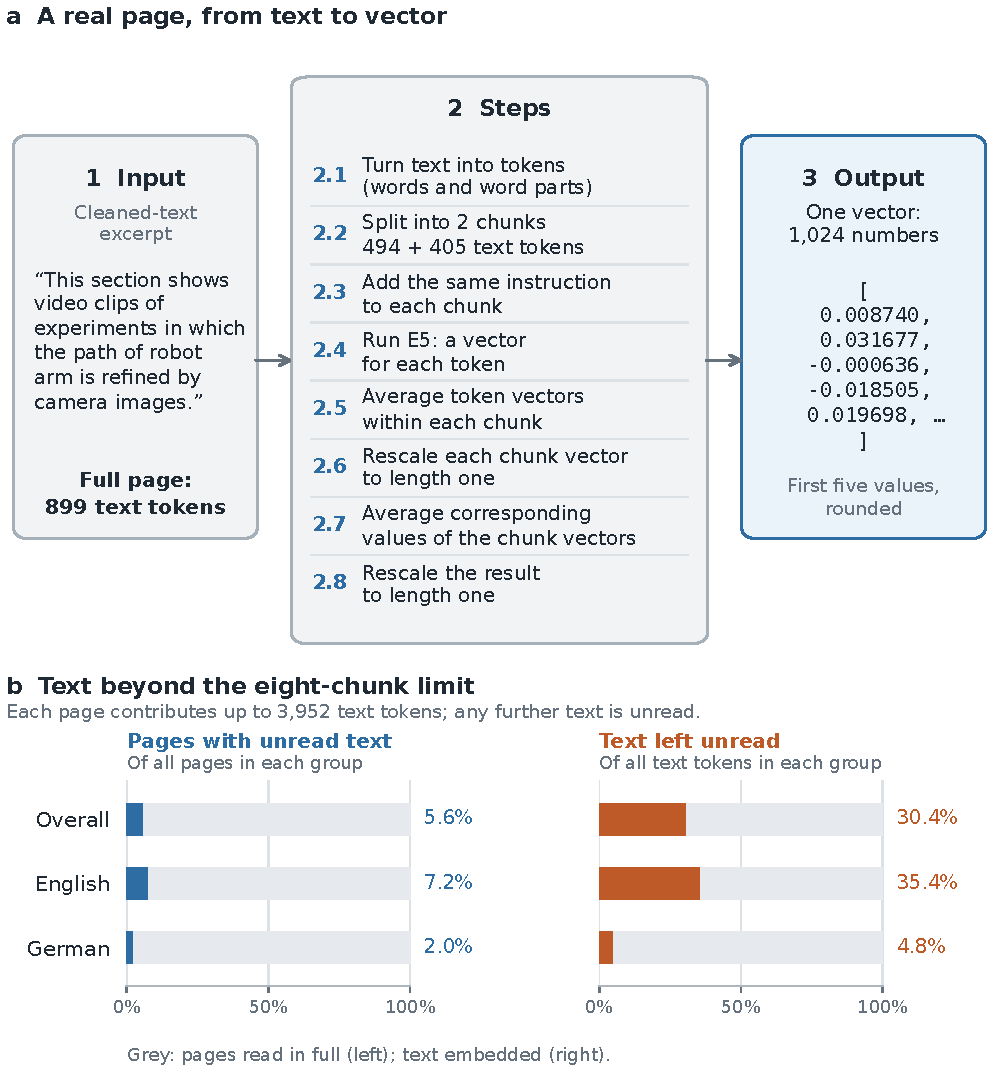
\includegraphics[width=\linewidth]{figs/fig_embedding_chunks.pdf}
\captionof{figure}{Chunking with E5. (a) \measured{} A real example using the robotics page
``Video Clips'' (saved crawl entry \texttt{eee5510b-60c1-4f6d-80e4-6a5f06cd3b2f}). The input is
an excerpt; the vector represents the full page. Only its first five values are shown, rounded
for display. The numbered steps separate tokenisation, E5 encoding and averaging. Rescaling
applies the same multiplier to every value in a vector.
(b) \measured{} Blue shows the percentage of pages with text beyond the limit. Orange shows
the percentage of all cleaned-text tokens beyond the limit. Overall, 5.6\% of pages have unread
text; their unread portions amount to 30.4\% of all text tokens because these pages are very
long. Each language row uses its own pages and text tokens.}
\label{fig:embedding-chunks}
\end{minipage}

E5 was chosen in part because it was trained to use task instructions, or prompts~\cite{wang2024multilingual}.
The aim was to guide the model towards research content and uncover topic structure hidden
in noisy web text.
% Exploratory evidence: output/stage2_lang/{eng,deu}/eval_results.json and
% output/stage2_lang_persona/{eng,deu}/eval_results.json.
\measured{} The limited prompt comparison in Section~\ref{sec:setaside-persona} did not
establish a consistent benefit from changing the instruction. Further prompt development was
not pursued because of time limits and because it was not needed to answer the three research
questions.

\subsection{Topic discovery with BERTopic}
\label{sec:method-bertopic}

Topic discovery runs separately for English and German on a sample of each language. Before
sampling, URL filters exclude page types such as code listings and catalogue pages from the
pool used to discover topics. These filters limit which documents shape discovery; the later
labeling step still covers the full corpus. The earlier model and language comparisons are
reported in Section~\ref{sec:setaside-models}.

BERTopic~\cite{grootendorst2022bertopic} receives the existing E5 vectors. UMAP
\cite{mcinnes2018umap} first reduces the number of coordinates used to represent each vector.
HDBSCAN~\cite{campello2013hdbscan} then finds dense groups: documents close together in that
reduced space. Documents that do not join a group receive the noise label $-1$.
The production setting uses \texttt{min\_topic\_size=100}, which sets the minimum cluster size;
the number of topics is not fixed in advance. Section~\ref{sec:rq3} examines that setting.

The groups receive descriptive keywords from their documents' cleaned body text. BERTopic
uses class-based TF-IDF, which scores words within each topic relative to the other topics.
The vectors determine the groups; the text supplies their descriptions. These discovered
topics are the input to document labeling. Figure~\ref{fig:bertopic-pipeline} shows these steps.

% Discovery flow in scripts/run_bertopic.py. Existing vectors are reused;
% cleaned text supplies the c-TF-IDF descriptions. The input example reuses the
% verified saved page and vector from Figure 5; the flow describes the full sample.
\noindent\begin{minipage}{\linewidth}
\centering
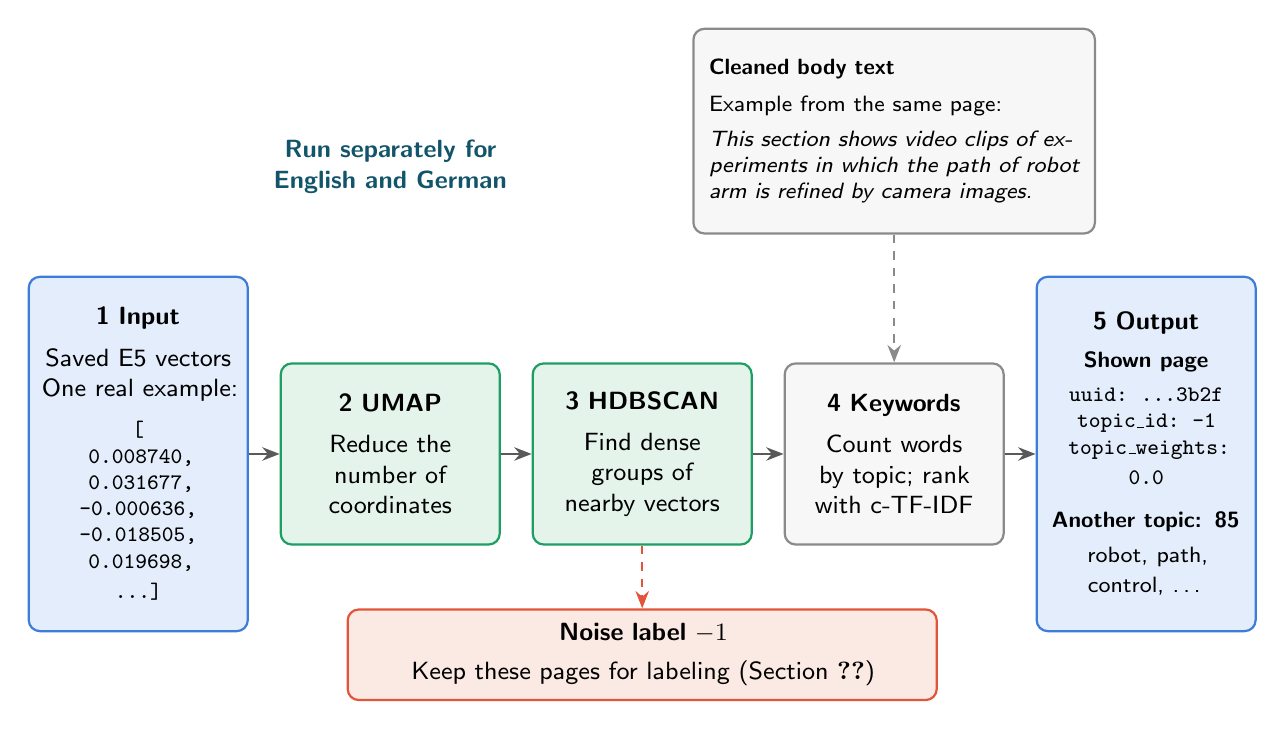
\begin{tikzpicture}[
  stage/.style = {rounded corners=4pt, draw, line width=0.8pt,
                  text width=2.50cm, minimum height=2.30cm,
                  align=center, inner xsep=4pt, inner ysep=5pt,
                  font=\small\sffamily},
  flow/.style = {-{Stealth[length=2.2mm,width=1.7mm]},
                 line width=0.9pt, draw=black!65},
  side/.style = {flow, dashed},
]

\node[font=\small\sffamily\bfseries, text=accent, align=center,
      text width=6.2cm] at (3.2,3.65)
  {Run separately for\\English and German};

\node[stage, minimum height=4.50cm, fill=fillblue, draw=boxblue] (input) at (0,0)
  {\textbf{1 Input}\\[4pt]
   Saved E5 vectors\\
   One real example:\\[5pt]
   {\footnotesize\ttfamily
    [\\
    0.008740,\\
    0.031677,\\
    -0.000636,\\
    -0.018505,\\
    0.019698,\\
    \ldots ]}};

\node[stage, fill=fillgreen, draw=boxgreen] (reduce) at (3.2,0)
  {\textbf{2 UMAP}\\[4pt]
   Reduce the\\number of\\coordinates};

\node[stage, fill=fillgreen, draw=boxgreen] (cluster) at (6.4,0)
  {\textbf{3 HDBSCAN}\\[4pt]
   Find dense\\groups of\\nearby vectors};

\node[stage, fill=black!3, draw=diagray] (words) at (9.6,0)
  {\textbf{4 Keywords}\\[4pt]
   Count words\\by topic; rank\\with c-TF-IDF};

\node[stage, minimum height=4.50cm, fill=fillblue, draw=boxblue] (output) at (12.8,0)
  {\textbf{5 Output}\\[4pt]
   {\footnotesize\textbf{Shown page}\\[3pt]
    \ttfamily
    uuid: ...3b2f\\
    topic\_id: -1\\
    topic\_weights:\\
    0.0}\\[6pt]
   {\footnotesize\textbf{Another topic: 85}\\[3pt]
    robot, path,\\
    control, \ldots}};

\draw[flow] (input.east) -- (reduce.west);
\draw[flow] (reduce.east) -- (cluster.west);
\draw[flow] (cluster.east) -- (words.west);
\draw[flow] (words.east) -- (output.west);

\node[stage, text width=4.70cm, minimum width=5.10cm,
      minimum height=2.60cm, fill=black!3, draw=diagray,
      align=left, font=\footnotesize\sffamily] (text) at (9.6,4.10)
  {\textbf{Cleaned body text}\\[4pt]
   Example from the same page:\\[3pt]
   \textit{This section shows video clips of experiments in which the path of robot arm
   is refined by camera images.}};
\draw[side, draw=diagray] (text.south) -- (words.north);

\node[stage, text width=7.20cm, minimum height=1.15cm,
      fill=fillred, draw=boxred] (noise) at (6.4,-2.55)
  {\textbf{Noise label $-1$}\\[3pt]
   Keep these pages for labeling (Section~\ref{sec:method-coverage})};
\draw[side, draw=boxred] (cluster.south) -- (noise.north);

\end{tikzpicture}
\captionof{figure}{BERTopic discovery on one language sample. \measured{} The input examples
reuse the robotics page from Figure~\ref{fig:embedding-chunks}: its saved vector and a
cleaned-text excerpt. Only the first five vector values are shown, rounded; the vector
represents the full page. All sampled pages are processed together. The displayed page
received $-1$ during discovery and continues to document labeling
(Section~\ref{sec:method-coverage}). Its output row comes from \texttt{doc\_topics.parquet},
with the page ID shortened here. The separate keyword example for topic 85 comes from
\texttt{topic\_top\_words.json} and describes other sampled pages.}
\label{fig:bertopic-pipeline}
\end{minipage}


\clearpage
\subsection{Document labeling}
\label{sec:method-coverage}

\begin{enumerate}[leftmargin=*,itemsep=0.4em]
\item \textbf{Calculate centroids.} Leave out $-1$ and sample pages flagged as code or data
dumps when forming the averages. For each topic with remaining sample pages, rescale its
vectors to length one, average them, then rescale the average to length one. This is the
topic's centroid, or centre.
\item \textbf{Calculate similarity scores.} Rescale each page vector to length one, then
compare it with every available centroid for its language using cosine similarity.
This score compares vector directions; a higher value means a closer match.
\item \textbf{Assign a topic.} Give each page the topic with the highest score. If scores tie,
choose the smallest topic ID.
\item \textbf{Save the label and flags.} Store the page ID, chosen topic, score, and the flags
for repeated website text and code/data pages.
\end{enumerate}

Figure~\ref{fig:labeling-pipeline} shows these steps with real input and output examples.

% Horizontal labeling flow, matching the discovery figure's style.
% Real example values are checked against the saved sample and production files.
\noindent\begin{minipage}{\linewidth}
\centering
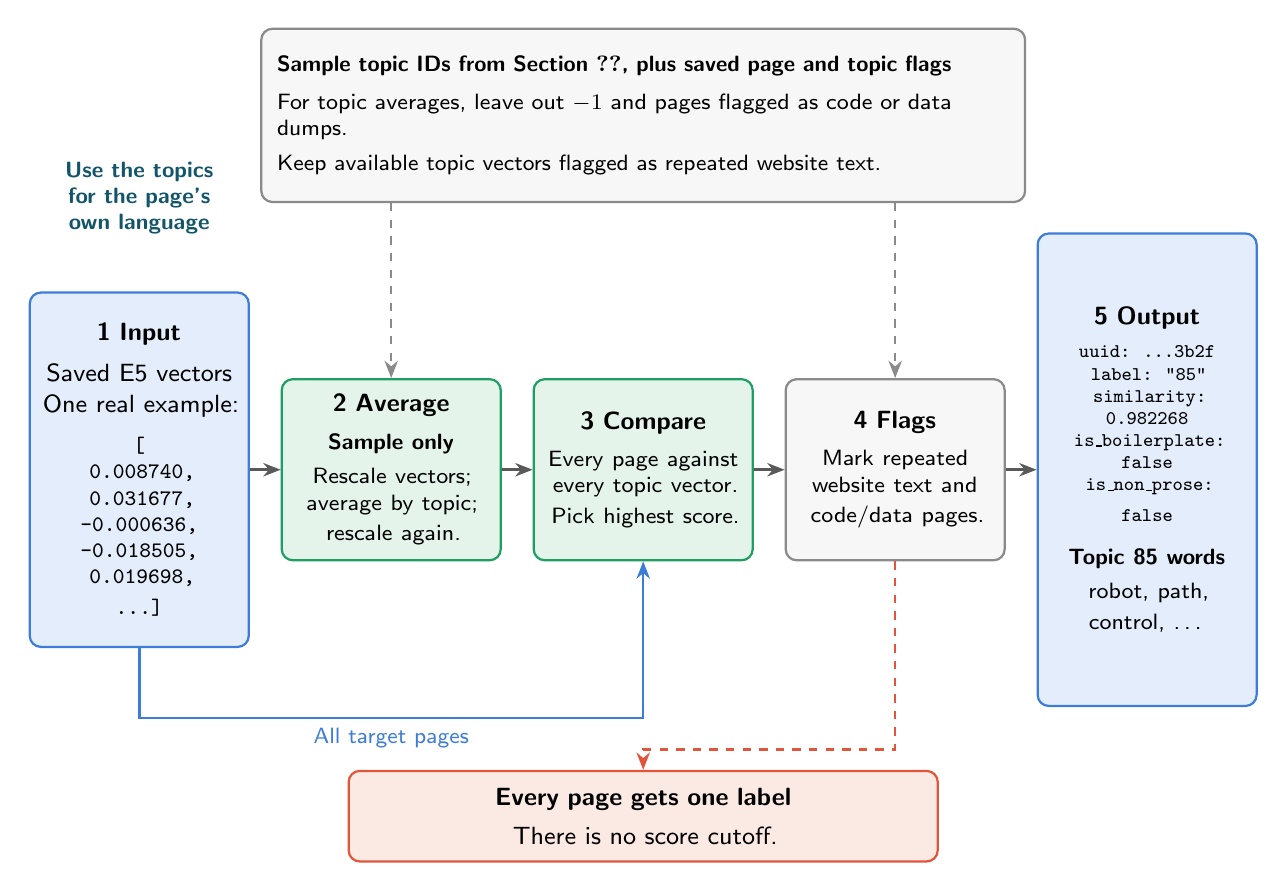
\begin{tikzpicture}[
  stage/.style = {rounded corners=4pt, draw, line width=0.8pt,
                  text width=2.50cm, minimum height=2.30cm,
                  align=center, inner xsep=4pt, inner ysep=5pt,
                  font=\small\sffamily},
  flow/.style = {-{Stealth[length=2.2mm,width=1.7mm]},
                 line width=0.9pt, draw=black!65},
  side/.style = {flow, dashed},
]

\node[font=\footnotesize\sffamily\bfseries, text=accent, align=center,
      text width=2.6cm] at (0,3.45)
  {Use the topics\\for the page's\\own language};

\node[stage, minimum height=4.50cm, fill=fillblue, draw=boxblue] (input) at (0,0)
  {\textbf{1 Input}\\[4pt]
   Saved E5 vectors\\
   One real example:\\[5pt]
   {\footnotesize\ttfamily
    [\\
    0.008740,\\
    0.031677,\\
    -0.000636,\\
    -0.018505,\\
    0.019698,\\
    \ldots ]}};

\node[stage, fill=fillgreen, draw=boxgreen] (average) at (3.2,0)
  {\textbf{2 Average}\\[4pt]
   {\footnotesize\textbf{Sample only}\\[3pt]
    Rescale vectors;\\
    average by topic;\\
    rescale again.}};

\node[stage, fill=fillgreen, draw=boxgreen] (compare) at (6.4,0)
  {\textbf{3 Compare}\\[4pt]
   {\footnotesize Every page against\\
    every topic vector.\\
    Pick highest score.}};

\node[stage, fill=black!3, draw=diagray] (flags) at (9.6,0)
  {\textbf{4 Flags}\\[4pt]
   {\footnotesize Mark repeated\\
    website text and\\
    code/data pages.}};

\node[stage, minimum height=6.00cm, fill=fillblue, draw=boxblue] (output) at (12.8,0)
  {\textbf{5 Output}\\[4pt]
   {\scriptsize\ttfamily
    uuid: ...3b2f\\
    label: "85"\\
    similarity:\\
    0.982268\\
    is\_boilerplate:\\
    false\\
    is\_non\_prose:\\
    false}\\[6pt]
   {\footnotesize\textbf{Topic 85 words}\\[3pt]
    robot, path,\\
    control, \ldots}};

\draw[flow] (input.east) -- (average.west);
\draw[flow] (average.east) -- (compare.west);
\draw[flow] (compare.east) -- (flags.west);
\draw[flow] (flags.east) -- (output.west);

\node[stage, text width=9.30cm, minimum width=9.70cm,
      minimum height=2.20cm, fill=black!3, draw=diagray,
      align=left, font=\footnotesize\sffamily] (metadata) at (6.4,4.50)
  {\textbf{Sample topic IDs from Section~\ref{sec:method-bertopic}, plus saved page and topic flags}\\[4pt]
   For topic averages, leave out $-1$ and pages flagged as code or data dumps.\\[3pt]
   Keep available topic vectors flagged as repeated website text.};

\draw[side, draw=diagray] (metadata.south -| average.north) -- (average.north);
\draw[side, draw=diagray] (metadata.south -| flags.north) -- (flags.north);

\draw[flow, draw=boxblue] (input.south) -- (0,-3.15) --
  node[below, font=\footnotesize\sffamily, text=boxblue] {All target pages}
  (6.4,-3.15) -- (compare.south);

\node[stage, text width=7.20cm, minimum height=1.15cm,
      fill=fillred, draw=boxred] (coverage) at (6.4,-4.40)
  {\textbf{Every page gets one label}\\[3pt]
   There is no score cutoff.};
\draw[side, draw=boxred] (flags.south) -- (9.6,-3.55) -| (coverage.north);

\end{tikzpicture}
\captionof{figure}{Document labeling from saved vectors to page labels.
\measured{} The robotics page from Figure~\ref{fig:embedding-chunks} was marked $-1$ in
Figure~\ref{fig:bertopic-pipeline} and receives topic 85 here.
Only its first five saved vector values are shown. The page ID, vector and word list are
abbreviated; the saved score is rounded. Sample vectors and topic averages are rescaled to
length one. Comparison uses vector directions; ties go to the smallest topic ID.
The flags mark repeated website text (\texttt{is\_boilerplate}) and code/data pages
(\texttt{is\_non\_prose}). Words describe the chosen topic. The saved row comes from
\texttt{doc\_labels.parquet} and the words from \texttt{topics.json}, under
\texttt{output/production\_labels/eng/}. Topic 85 was not later divided.}
\label{fig:labeling-pipeline}
\end{minipage}

\clearpage

% --------------------------------------------------------- EXPERIMENTAL DESIGN
\section{Experimental design}
\label{sec:experimental-design}

The experiments were designed to answer the three research questions and guide the development
of the pipeline. Clustering and labeling methods were compared to determine which to use at
each step.

This section also explains why the benchmarks described in Section~\ref{sec:method-benchmarks}
were chosen and how they are used to assess the pipeline. Their known categories provide a
reference for judging how well the discovered groups and the final page labels match known
topics.

\subsection{Clustering}
\label{sec:experiment-comparisons}

The initial comparison tested BERTopic~\cite{grootendorst2022bertopic}, LDA~\cite{blei2003lda},
a local S\textsuperscript{3} baseline~\cite{kardos2025s3}, FASTopic~\cite{wu2024fastopic},
CombinedTM~\cite{bianchi2021combinedtm} and TopicGPT-Lite, a local adaptation of
TopicGPT~\cite{pham2024topicgpt}. The models were tested on separate English and German
samples of the DLR crawl. The comparisons considered word coherence, coverage and cluster
separation (Section~\ref{sec:method-metrics}), alongside the topic counts and keyword lists.

The DLR experiments gave no clear basis for choosing a topic count (Section~\ref{sec:rq1-nok}).
The crawl mixes many subjects with repeated navigation text and page templates
(Section~\ref{sec:method-corpus}). A cluster of pages that share a template can score well on
word coherence because it repeats the same terms. The same models were tested on the GDELT control described
in Section~\ref{sec:method-benchmarks}. Because the articles cover one event, the flood and
the response to it, a small number of topics was expected.

\measured{} The separate silhouette sweep in Figure~\ref{fig:gdelt-silhouette} scored two groups
highest among the tested counts. BERTopic also returned two groups in the corrected GDELT run
(Figure~\ref{fig:gdelt-models}).

\noindent\begin{minipage}{\linewidth}
\centering
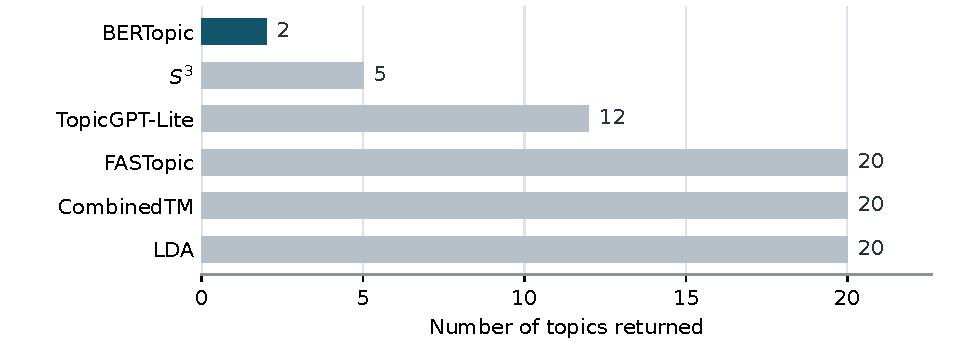
\includegraphics[width=0.93\linewidth]{figs/fig_gdelt_models.pdf}
\captionof{figure}{Topic counts on the GDELT flood corpus. \measured{} The bars show topics
with assigned articles in the corrected run, excluding noise. BERTopic used a minimum cluster
size of 100. S3 returned the lowest count in its search range.
TopicGPT-Lite was asked for 20 topics. FASTopic, CombinedTM and LDA were set to 20.
Source \texttt{output/gdelt\_ahrtal\_v2/}\allowbreak\texttt{eval\_results.json}.}
\label{fig:gdelt-models}
\end{minipage}

The GDELT result supported the choice of BERTopic for the pipeline. Using the E5 vectors,
it returned few groups on the focused control and many fine topics on the DLR crawl
without a preset topic count. Its keywords make the topics easier to inspect
(Section~\ref{sec:method-bertopic}). Another reason for choosing BERTopic was its
\texttt{min\_topic\_size} setting, which controls how small a cluster can be. RQ3 varies this
setting to test how coarse or fine the topics should be, using LDA as a fixed coarse reference
(Section~\ref{sec:rq3-hierarchy}).

\subsection{Document labeling}
\label{sec:experiment-labeling}

The first labeling experiment followed a suggestion from the OpenSearch@DLR~1.0 team to use an
existing labeling model with its own embeddings. Lbl2Vec~\cite{schopf2021lbl2vec} was tested
with BERTopic's keywords. It trained a separate Doc2Vec~\cite{le2014doc2vec} model on each
benchmark and used the keywords to find documents from which to build topic vectors.
Its 300-dimensional Doc2Vec vectors occupied a different embedding space from the
1{,}024-dimensional E5 vectors that BERTopic had clustered.

Once BERTopic had found the clusters, the task was to assign each document to one of them.
This motivated comparing each document with the cluster centroids in the same E5 space
(Section~\ref{sec:method-coverage}). The comparisons run on a CPU using the saved E5 vectors,
which avoids the cost of training and running a second embedding model.

The original BERTopic clusters give the reference score before labeling. \measured{} They had
the highest NMI on each benchmark in Figure~\ref{fig:labeling-benchmarks}. Nearest centroid
stayed closer to that score than Lbl2Vec did. Lbl2Vec changed both the embedding model and
the way topics were represented, so this comparison cannot isolate how much of the loss
came from switching to Doc2Vec.

\noindent\begin{minipage}{\linewidth}
\centering
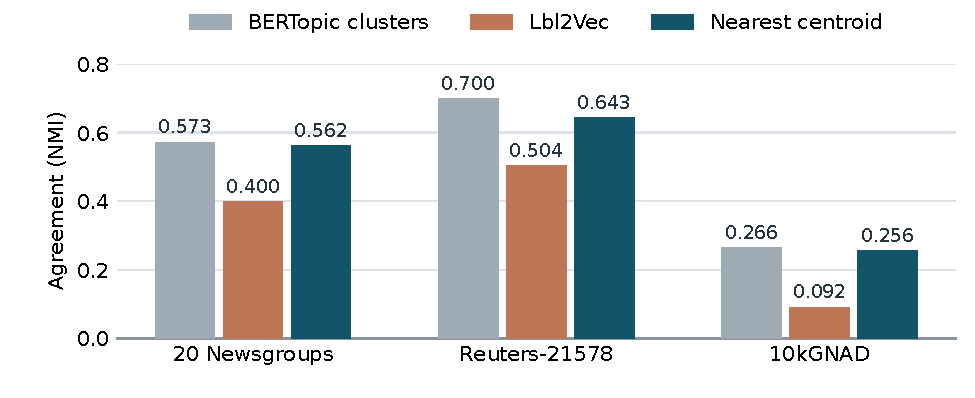
\includegraphics[width=0.98\linewidth]{figs/fig_labeling_benchmarks.pdf}
\captionof{figure}{Agreement with known classes before and after labeling, measured by NMI
(Section~\ref{sec:method-metrics}). \measured{} Within each benchmark all three scores use the
same documents, with BERTopic noise excluded and minimum cluster size fixed at 100.
Sources \texttt{data/groundtruth/} and \texttt{output/groundtruth/}.}
\label{fig:labeling-benchmarks}
\end{minipage}

\measured{} Across the prepared benchmarks, Lbl2Vec returned labels for about 93\% of documents
on each English benchmark and 99.8\% on 10kGNAD. Nearest centroid labeled every document that
reached the labeling step. This covered 99.5\% of 20 Newsgroups and 100\% of the other two
benchmarks. These results led to the choice of nearest centroid for the pipeline.

\subsection{Evaluation measures}
\label{sec:method-metrics}

The evaluation measures were chosen to assess how coherent and distinct the topics are and
how well the clusters are separated. They also show whether every document receives a label
and how closely the assigned labels match the known classes on the benchmarks.

\begin{description}[leftmargin=1.3em,style=nextline,itemsep=3pt]
\item[Word coherence from NPMI.]
Normalised pointwise mutual information (NPMI) scores topic word lists from text
alone~\cite[p.~533]{lau2014tealeaves}. It was chosen so that models could be compared on the
unlabelled DLR crawl using the same reference text.

NPMI checks whether two words appear together more
often than expected from how common each word is on its own~\cite[Eq.~(7)]{bouma2009npmi}.
The reference text is read in short stretches called windows, each up to $h$ tokens long.
For two words $u$ and $v$, $p_h(u)$ and $p_h(v)$ are the shares of windows with each word.
The share of windows with both words is $p_h(u,v)$. The pair score is
\[
  f_h(u,v)=
  \frac{\log\!\bigl((p_h(u,v)+\varepsilon)/(p_h(u)p_h(v))\bigr)}
       {-\log\!\bigl(p_h(u,v)+\varepsilon\bigr)},
\]
where the small number $\varepsilon=10^{-12}$ lets the formula work even when the two words
never appear together.

\emph{Example.} Suppose \emph{ice} and \emph{hockey} each appear in 20 out of 100 windows.
If they appeared independently, both would be expected in $100\times0.20\times0.20=4$ windows.
Suppose they actually appear together in 10. Putting these counts into the formula gives an
NPMI of about $0.40$. The score is positive because the words appear together more often
than expected.

To score a topic, take the average over all pairs of its $m$ top words
$W=(w_1,\ldots,w_m)$. This evaluation uses 10-token windows~\cite[Table~2]{roder2015coherence}.
\[
  \mathrm{NPMI}(W)=\frac{2}{m(m-1)}\sum_{1\le i<j\le m}f_{10}(w_i,w_j).
\]

\item[Word coherence from $C_v$.]
$C_v$ was used as a second check on whether a topic's words fit together. It checks how well
each word fits the pattern of the whole list~\cite[Eqs.~(34)--(35) and Table~2]{roder2015coherence}.

For each word $w$, use the NPMI formula to score it with every word $u$ in the topic list
$W$, including itself. Use 110-token windows. Write the scores as a vector
$v_w=(f_{110}(w,u))_{u\in W}$. Add the word vectors to get $v_W=\sum_{w\in W}v_w$.
Compare each $v_w$ with $v_W$ using cosine similarity and average the results over the
$m$ words. The notation $\|\cdot\|_2$ means vector length.
\[
  C_v(W)=\frac{1}{m}\sum_{w\in W}
  \frac{v_w\cdot v_W}{\|v_w\|_2\,\|v_W\|_2}.
\]

\emph{Example.} Suppose \emph{ice} and \emph{hockey} appear in the same 20 out of 100 windows.
The word \emph{printer} also appears in 20 windows and shares four with the other two words.
In the order \emph{ice}, \emph{hockey}, \emph{printer}, the rounded vectors are
$(1,1,0)$ for both \emph{ice} and \emph{hockey}, and $(0,0,1)$ for \emph{printer}.
Their sum is $(2,2,1)$. Compared with the sum, the first two words score about $0.94$ each,
and \emph{printer} scores about $0.33$. The average gives $C_v\approx0.74$.

Both coherence measures use up to ten words per topic. The evaluation drops words outside
its reference vocabulary and skips topics left with fewer than two words. Each model's
score is the mean across the remaining topics, with higher values indicating stronger
coherence (\texttt{scripts/run\_eval.py}).

\item[Topic diversity.]
Topics can score well on coherence and still use many of the same words. Topic diversity
was chosen to check for this repetition across topics.

Make one list $L$ with up to ten top words from each topic
(\texttt{scripts/}\allowbreak\texttt{eval\_junk\_filtered.py}). Divide the number of different
words in $L$ by $|L|$, the number of entries including repeats~\cite[p.~448]{dieng2020etm}.
\[
  \mathrm{Diversity}=\frac{|\{w:w\in L\}|}{|L|}.
\]
A higher value means less repetition between topic descriptions.

\emph{Example.} Suppose one topic lists \emph{ice}, \emph{hockey} and \emph{skates}.
Another lists \emph{ice}, \emph{snow} and \emph{winter}. There are six entries and five
different words because \emph{ice} appears twice. The diversity is $5/6\approx0.83$.

\item[Coverage.]
Let $N_{\mathrm{input}}$ be the number of input documents and $N_{\mathrm{labelled}}$ the
number that receive a topic. Coverage checks the requirement in
Section~\ref{sec:intro-neutrality}.
\[
  \mathrm{Coverage}(\%)=100\,\frac{N_{\mathrm{labelled}}}{N_{\mathrm{input}}}.
\]

\item[Silhouette.]
For document $i$, let $a_i$ be the mean cosine distance to the other documents in its
cluster. Let $b_i$ be the smallest mean distance to the documents of any other cluster.
The overall score averages the individual scores over the $n$ evaluated documents
\cite[pp.~55--56,~59]{rousseeuw1987silhouette}.
\[
  s_i=\frac{b_i-a_i}{\max(a_i,b_i)},\qquad
  \mathrm{Silhouette}=\frac{1}{n}\sum_{i=1}^{n}s_i.
\]
A document alone in its cluster contributes zero. Higher values indicate better separation.

\item[Davies--Bouldin index.]
Let $K$ be the number of evaluated clusters, $\mu_k$ the mean vector of cluster $k$, and
$S_k$ the mean Euclidean distance of its document vectors to $\mu_k$. The denominator
$\|\mu_k-\mu_\ell\|_2$ is the Euclidean distance between the two cluster centres.
For each cluster $k$, the index takes the worst ratio of spread to separation over the
other clusters $\ell$ and then averages these ratios~\cite[p.~225]{davies1979cluster}.
\[
  \mathrm{DB}=\frac{1}{K}\sum_{k=1}^{K}
  \max_{\ell\ne k}\frac{S_k+S_\ell}{\|\mu_k-\mu_\ell\|_2}.
\]
Lower values indicate better separation. The model comparison computes both geometry
scores on sampled documents in the shared UMAP evaluation space
(\texttt{scripts/run\_eval.py}).

\item[Agreement with reference labels.]
Let $\Omega$ be the assignment to clusters $\omega_1,\ldots,\omega_K$, and let $C$ be
the reference classification into classes $c_1,\ldots,c_J$ on the same $N$ scored
documents. Write $p_k=|\omega_k|/N$ and $q_j=|c_j|/N$ for the cluster and class shares.
Write $p_{kj}=|\omega_k\cap c_j|/N$ for the share in both. The entropies $H(\Omega)$
and $H(C)$ measure uncertainty in cluster and class membership, and mutual information
$I$ measures how much they tell us about each other.
\[
\begin{aligned}
  H(\Omega)&=-\sum_{k=1}^{K}p_k\log p_k,&
  H(C)&=-\sum_{j=1}^{J}q_j\log q_j,\\
  I&=\sum_{k=1}^{K}\sum_{j=1}^{J}p_{kj}\log\frac{p_{kj}}{p_kq_j}. &&
\end{aligned}
\]
Terms with $p_{kj}=0$ contribute zero to $I$. Normalised mutual information (NMI)
divides $I$ by the mean of the two entropies. Adjusted mutual information (AMI) also
subtracts the expected mutual information $E[I]$ under random assignments with the
same cluster and class sizes~\cite[Table~2, p.~2841 and Sec.~4.1]{vinh2010information}.
\[
  \mathrm{NMI}=\frac{I}{\tfrac12[H(\Omega)+H(C)]},\qquad
  \mathrm{AMI}=\frac{I-E[I]}{\tfrac12[H(\Omega)+H(C)]-E[I]}.
\]
Purity counts the documents in the most common reference class of each cluster and
divides by $N$~\cite[Eq.~(16.1), p.~357]{manning2008ir}.
\begin{equation}
  \mathrm{Purity}=\frac{1}{N}\sum_{k=1}^{K}\max_{1\le j\le J}|\omega_k\cap c_j|.
  \label{eq:benchmark-purity}
\end{equation}
Higher values indicate greater agreement. All three scores are calculated only on
labelled benchmarks (\texttt{scripts/run\_groundtruth\_metrics.py}).

\item[Elapsed time.]
For a timed operation, $t_{\mathrm{start}}$ and $t_{\mathrm{end}}$ are the clock
readings immediately before and after it. This measure is used for the exploratory
search experiments in Section~\ref{sec:setaside-speed}.
\[
  t_{\mathrm{elapsed}}=t_{\mathrm{end}}-t_{\mathrm{start}}.
\]
\end{description}

Ground-truth scores use the documents available in both a run's output and the prepared
reference labels. Raw BERTopic scores exclude the noise label $-1$. Different runs can
therefore be scored on different document sets; coverage must be read alongside agreement
scores. The largest-class baseline for purity must also be calculated on the set actually
scored.

The language-model judge used in earlier exploration is excluded from this evaluation panel.

\subsection{The purity floor}
\label{sec:experimental-purity-floor} \proved{} Purity can never
fall below the share of the largest class, provided every document carries exactly one class and is
placed in exactly one cluster. Figure~\ref{fig:purityfloor} shows the argument on a ten-document example.
Use the purity definition in Equation~\eqref{eq:benchmark-purity} and let $c^\ast$ be
the largest reference class.
\begin{enumerate}[leftmargin=1.5em,itemsep=2pt]
\item \emph{Inside one cluster.} The largest class count inside a cluster must be at least the
count belonging to $c^\ast$:
\[
  \max_j |\omega_k \cap c_j| \;\ge\; |\omega_k \cap c^\ast| \qquad \text{for every } k.
\]
\item \emph{Adding over clusters.} Add this inequality over all clusters and divide by $N > 0$:
\[
  \text{purity} \;\ge\; \frac{1}{N}\sum_{k=1}^{K} |\omega_k \cap c^\ast|.
\]
\item \emph{Counting the largest class.} Each document in $c^\ast$ belongs to exactly one
cluster, so these counts add up to $|c^\ast|$:
\[
  \sum_{k=1}^{K} |\omega_k \cap c^\ast| \;=\; |c^\ast|.
\]
\end{enumerate}
Together, $\text{purity} \ge |c^\ast|/N$. Putting every document in one cluster reaches this bound
exactly, so it cannot be raised. Any clustering that places every document therefore scores at
least $0.4887$ on Reuters, but only $0.0544$ on 20 Newsgroups (Section~\ref{sec:neutrality}).

\begin{figure}[t]\centering
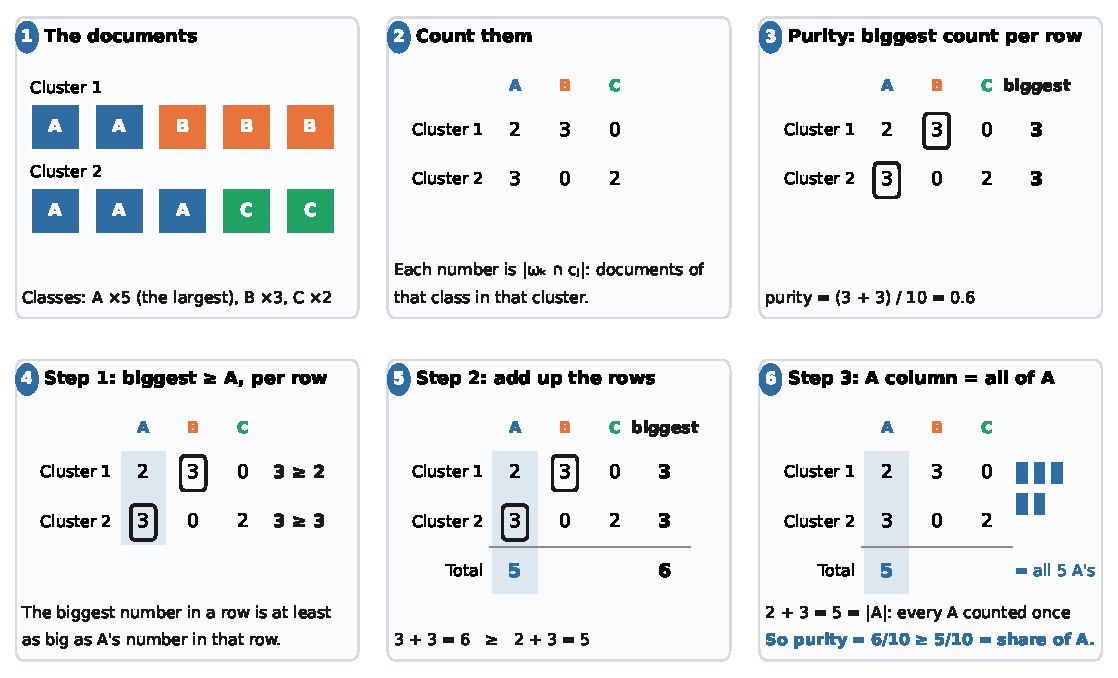
\includegraphics[width=\textwidth]{figs/fig_purity_floor}
\caption{Visual proof of the purity floor, one step per panel, on ten documents with classes A
(5 documents, the largest), B (3) and C (2). \textbf{(1)}~The documents in two clusters.
\textbf{(2)}~The same clustering as counts, one row per cluster. \textbf{(3)}~Purity adds the
biggest count in each row (boxed). \textbf{(4)--(6)}~The three steps of the proof: in each row the
boxed count is at least A's count (shaded); adding up the rows keeps the inequality; and the A
column adds up to all of A.}
\label{fig:purityfloor}
\end{figure}


\clearpage
% Working outline: old prose cleared on 2026-11-09.
\section{RQ1 --- Discovering fine topics with nothing labelled}
\label{sec:rq1}

\subsection{The result}

\subsection{There is no natural number of topics in this corpus}
\label{sec:rq1-nok}

\subsection{What it gets wrong: junk topics, and the metric that cannot see them}
\label{sec:rq1-junk}

\subsection{Answer to RQ1}


% Working outline: old prose cleared on 2026-11-09.
\section{RQ2 --- Which feature should be embedded?}
\label{sec:rq2}

\subsection{The question and the design}

\subsection{Reading the table}

\subsection{A note on how this answer changed}

\subsection{Answer to RQ2}


% Working outline: old prose cleared on 2026-11-09.
\section{RQ3 --- How much granularity is enough?}
\label{sec:rq3}

\subsection{Why this needs a new criterion}

\subsection{Building the coarse--fine hierarchy}
\label{sec:rq3-hierarchy}

For this analysis, LDA supplies a fixed coarse reference and BERTopic supplies the fine
topics. The models are fitted on the same sample for each language. The script
\texttt{build\_topic\_hierarchy.py} selects a candidate parent for each fine topic: the coarse
topic containing the largest share of its documents. It checks this share and the lead over
the next-best parent. It also checks whether centroid similarity favours the same parent and
whether the child is among that parent's largest document contributors.

A link is rejected when overlap is weak, the candidate parents are nearly tied, or the
centroid and reverse checks jointly oppose the candidate. A confidence score records
agreement between these signals. The children counted below are those with accepted links;
the rules are held fixed across the sweep. The saved mappings are in
\texttt{output/hierarchy\_probe/}. Rejecting a link leaves a fine topic without an accepted
coarse parent; it does not remove documents or change their production labels.

\subsection{The floor: a split needs at least two children}

\subsection{The sweep}

\subsection{What the sweep shows}

\subsection{Why the floor alone cannot select a setting}
\label{sec:rq3-floorlimit}

\subsection{The ceiling: do the children differ from one another?}
\label{sec:rq3-ceiling}

\subsection{Both bounds at once: counting real splits}
\label{sec:rq3-joint}

\subsection{Which of the two measures actually locates a setting}
\label{sec:rq3-null}

\subsection{What this does to the German answer}
\label{sec:rq3-german}

\subsection{Answer to RQ3}


% Working outline: old prose cleared on 2026-11-09.
\section{Testing data neutrality}
\label{sec:neutrality}

\subsection{What has to be shown}

\subsection{A confound that had to be fixed first}
\label{sec:neutrality-confound}

\subsection{The transfer result}

\subsection{Is the purity inflated by over-clustering?}

\subsection{The assignment stage, measured against labels}
\label{sec:neutrality-centroid}

\subsection{What this does and does not establish}


% Working outline: old prose cleared on 2026-11-09.
\section{Explored and set aside}
\label{sec:setaside}

\subsection{Four topic models that did not survive benchmarking}
\label{sec:setaside-models}

English and German use separate topic-discovery runs. \measured{} An earlier mixed-language run
produced mostly topics containing almost only English or almost only German documents.\footnote{
In the combined-language BERTopic runs, approximately 72--75\% of topics
had at least 95\% of their documents in one language. Noise assignments were excluded.
The diagnostic is saved in \texttt{output/stage2\_clean/}\allowbreak\texttt{lang\_purity\_report.json}.}
This motivated separate models.

\subsection{A separate cross-granularity matching diagnostic}
\label{sec:method-crossgran}

This exploratory diagnostic compares coarse LDA topics with fine BERTopic topics. It is
separate from the hierarchy used for RQ3 (Section~\ref{sec:rq3-hierarchy}) and leaves production
labels unchanged. For each fine topic $f$, its candidate parent $c$ is the coarse topic with
the largest document overlap. This adapts the pairing-strength idea from Bidirectional Topic
Matching~\cite[p.~4, Eq.~(1)]{adam2024btm}.

The script pairs the two models' assignments by page identifier. Overlap uses the resulting
rows carrying non-noise labels from both models; repeated rows are retained. It is the share
of those rows in $f$ whose coarse label is $c$.
The \emph{lead} is the largest overlap minus the second-largest overlap, with a missing
second share treated as zero. The candidate pair receives the weighted score

\begin{equation}
\mathrm{conf}(f, c) \;=\; 0.5 \cdot \mathrm{overlap}(f,c) \;+\; 0.3 \cdot \mathrm{sim}(f,c)
\;+\; 0.2 \cdot \mathrm{bidir}(f,c)
\end{equation}

where $\mathrm{sim}$ is the cosine similarity between the two topic centroids. For each coarse
topic, fine topics are ranked by overlap multiplied by their number of rows in the paired
assignments. The indicator $\mathrm{bidir}$ is one when $f$ ranks among the top three for $c$, and zero
otherwise. This is the contribution check used by the script.

As in TopicCheck~\cite[pp.~177--178]{chuang2015topiccheck}, a topic may remain without an
accepted match. This diagnostic applies its checks in the following order:
\begin{enumerate}[leftmargin=1.6em,itemsep=2pt]
\item \textsc{Reject} if overlap is below $0.35$ or similarity is below $0.25$.
\item Otherwise, mark \textsc{ambiguous} if the lead is below $0.25$.
\item Otherwise, mark \textsc{low confidence} if the weighted score is below $0.45$.
\item Otherwise, accept the candidate as a \textsc{match}.
\end{enumerate}

\begin{table}[h]\centering
\caption{Outcomes of the separate matching diagnostic at \texttt{min\_topic\_size=100}.
Each fine topic contributes one decision.}
\label{tab:crossgran}
\begin{tabular}{lrrrr}
\toprule
Language & \textsc{match} & \textsc{ambiguous} & \textsc{low conf.} & \textsc{reject} \\
\midrule
English & 99 & 12 & 0 & 1 \\
German  & 69 & 4  & 0 & 5 \\
\bottomrule
\end{tabular}
\end{table}

\measured{} The saved candidate-parent similarities range from $0.8927$ to $0.9993$ in English
and from $0.9300$ to $0.9991$ in German. These ranges describe the parent selected for each fine
topic. The saved files do not contain similarities for every possible fine--coarse pair.\footnote{\raggedright
Ranges, score minima and decision counts are recomputed from
\texttt{output/crossgran/}\allowbreak\texttt{crossgran\_\{eng,deu\}.json}.
Each file stores one record per fine topic.}

\measured{} No saved candidate failed the similarity check. Every rejection in
Table~\ref{tab:crossgran} was caused by insufficient overlap. Among candidates reaching the
weighted-score check, the lowest score was $0.5617$ in English and $0.4952$ in German.
Both exceed its cutoff, explaining the empty \textsc{low confidence} category. A
\textsc{match} label means only that the candidate passed these checks.

\subsection{Automatically generated keywords versus a human keyword list}
\label{sec:setaside-keywords}

\subsection{Search speed: a real engineering result with no research claim}
\label{sec:setaside-speed}

\subsection{A hyperlink topic graph}
\label{sec:setaside-graph}

\subsection{Category-filtered search, and why it cannot support a quality claim}
\label{sec:setaside-utility}

\subsection{Persona prompting the embedder}
\label{sec:setaside-persona}

A persona instruction asks the model to adopt a role. An earlier comparison used the role of
a research librarian. The motivation is given in Section~\ref{sec:method-embed}. The two
instructions were:

\begin{description}[leftmargin=1.3em,style=nextline,itemsep=3pt]
\item[Original.] ``Identify the main research topic of this web page''
\item[Librarian.] ``You are an expert research librarian. Identify the specific scientific
research theme of this web page.''
\end{description}

These were exploratory runs before the final production setup. Each language sample contained
50{,}000 entries, including some repeated pages. BERTopic used
\texttt{min\_topic\_size=100} throughout. Table~\ref{tab:prompt-comparison} reports the saved scores after
pages initially left outside any topic had been reassigned. Every sampled entry then received
a topic.\footnote{\raggedright Scores are from
\texttt{output/stage2\_lang/}\allowbreak\texttt{\{eng,deu\}/}\allowbreak\texttt{eval\_results.json}
and \texttt{output/stage2\_lang\_persona/}\allowbreak\texttt{\{eng,deu\}/}\allowbreak\texttt{eval\_results.json},
entry \texttt{BERTopic-min100-reduced}. Sample identities are stored in
\texttt{sample\_data/sample\_data.parquet} under each language directory.}
The scores are defined in Section~\ref{sec:method-metrics}. Word coherence used each run's
sample texts. Silhouette used 10{,}000 sampled entries after UMAP reduced the vectors to
50 coordinates.

\noindent\begin{minipage}{\linewidth}
\centering
\captionof{table}{Earlier instruction comparison after reassignment. \emph{Topics} gives the
number of discovered groups. Higher values are better for NPMI, $C_v$ and silhouette.}
\label{tab:prompt-comparison}
\begin{tabular}{llrrrr}
\toprule
Language & Instruction & Topics & NPMI & $C_v$ & Silhouette \\
\midrule
English & Original  & 110 & $-0.138$ & 0.429 & $-0.082$ \\
English & Librarian & 109 & $-0.143$ & 0.464 & $-0.037$ \\
German  & Original  &  77 & $-0.238$ & 0.402 & $-0.130$ \\
German  & Librarian &  70 & $-0.251$ & 0.352 & $-0.227$ \\
\bottomrule
\end{tabular}
\end{minipage}

\measured{} With the librarian instruction, English $C_v$ and silhouette are higher, while
NPMI is lower. In German, all three scores are lower. The changes therefore show no consistent
gain across the scores and languages. German coherence covers only 65 of the original run's
77 topics and 59 of the librarian run's 70 topics. The other topics had too few words in the
evaluation vocabulary, the list retained for coherence scoring.

The comparison has important limits. \measured{} The saved samples contain different pages
and include repeated entries. Comparing their page identifiers gives 7{,}809 shared distinct
English pages and 20{,}789 shared distinct German pages. The longer instruction also leaves
less room for page text in each chunk.
These differences prevent isolating the effect of instruction wording. This comparison covers
one alternative instruction and does not establish that other prompts would fail.


% Working outline: old prose cleared on 2026-11-09.
\section{Failure log and retractions}
\label{sec:failures}

\subsection{Retractions}

\subsection{Defects and corrections that were not claims}

\subsection{Two patterns worth generalising}


% Working outline: old prose cleared on 2026-11-09.
\section{Limitations and threats to validity}
\label{sec:limitations}

\subsection{Limitations of the main result}

\subsection{Limitations of the evaluation}

\subsection{Limitations of the system}

\subsection{Threats to the data-neutrality argument}


% Working outline: old prose cleared on 2026-11-09.
\section{Conclusion}
\label{sec:conclusion}

\subsection{What was asked and what was found}

\subsection{The argument in one paragraph}

\subsection{What this work contributes}

\subsection{What should be done next}

\subsection{Closing}


% Working outline: old prose cleared on 2026-11-09.
\appendix
\section{Implementation index}
\label{sec:appendix-code}

\section{Reproducing the tables}

\begin{thebibliography}{99}
\addcontentsline{toc}{section}{References}

% ---------------------------------------------------------------- models
\bibitem{blei2003lda}
D.~M. Blei, A.~Y. Ng, and M.~I. Jordan.
\newblock Latent Dirichlet Allocation.
\newblock \emph{Journal of Machine Learning Research}, 3:993--1022, 2003.

\bibitem{grootendorst2022bertopic}
M.~Grootendorst.
\newblock BERTopic: Neural topic modeling with a class-based TF-IDF procedure.
\newblock arXiv:2203.05794, 2022.

\bibitem{kardos2025s3}
M.~Kardos, J.~Kostkan, K.~Enevoldsen, A.-Q.~Vermillet, K.~Nielbo, and R.~Rocca.
\newblock S\textsuperscript{3} -- Semantic Signal Separation.
\newblock In \emph{Proceedings of the 63rd Annual Meeting of the Association for Computational
Linguistics (ACL)}, pages 633--666, 2025. \url{https://aclanthology.org/2025.acl-long.32/}.

\bibitem{wu2024fastopic}
X.~Wu, T.~Nguyen, D.~C. Zhang, W.~Y. Wang, and A.~T. Luu.
\newblock FASTopic: Pretrained Transformer is a Fast, Adaptive, Stable, and Transferable Topic Model.
\newblock In \emph{Advances in Neural Information Processing Systems (NeurIPS)}, volume~37,
pages 84447--84481, 2024.
\url{https://doi.org/10.52202/079017-2683}.

\bibitem{bianchi2021combinedtm}
F.~Bianchi, S.~Terragni, and D.~Hovy.
\newblock Pre-training is a Hot Topic: Contextualized Document Embeddings Improve Topic Coherence.
\newblock In \emph{Proceedings of ACL-IJCNLP}, volume~2, pages 759--766, 2021.
\url{https://aclanthology.org/2021.acl-short.96/}.

\bibitem{pham2024topicgpt}
C.~M. Pham, A.~Hoyle, S.~Sun, P.~Resnik, and M.~Iyyer.
\newblock TopicGPT: A Prompt-based Topic Modeling Framework.
\newblock In \emph{Proceedings of NAACL-HLT}, volume~1, pages 2956--2984, 2024.
\url{https://aclanthology.org/2024.naacl-long.164/}.

\bibitem{mcinnes2018umap}
L.~McInnes, J.~Healy, and J.~Melville.
\newblock UMAP: Uniform Manifold Approximation and Projection for Dimension Reduction.
\newblock arXiv:1802.03426, 2018.

\bibitem{campello2013hdbscan}
R.~J.~G.~B. Campello, D.~Moulavi, and J.~Sander.
\newblock Density-Based Clustering Based on Hierarchical Density Estimates.
\newblock In \emph{Advances in Knowledge Discovery and Data Mining (PAKDD)}, pages 160--172, 2013.

\bibitem{wang2024multilingual}
L.~Wang, N.~Yang, X.~Huang, L.~Yang, R.~Majumder, and F.~Wei.
\newblock Multilingual E5 Text Embeddings: A Technical Report.
\newblock arXiv:2402.05672, 2024.

\bibitem{dieng2020etm}
A.~B. Dieng, F.~J.~R. Ruiz, and D.~M. Blei.
\newblock Topic Modeling in Embedding Spaces.
\newblock \emph{Transactions of the Association for Computational Linguistics}, 8:439--453, 2020.

% ------------------------------------------------- hierarchy and matching
\bibitem{zhang2018taxogen}
C.~Zhang, F.~Tao, X.~Chen, J.~Shen, M.~Jiang, B.~Sadler, M.~Vanni, and J.~Han.
\newblock TaxoGen: Unsupervised Topic Taxonomy Construction by Adaptive Term Embedding and
Clustering.
\newblock In \emph{Proceedings of KDD}, pages 2701--2709, 2018. arXiv:1812.09551.

\bibitem{shahid2023hyhtm}
S.~Shahid, T.~Anand, N.~Srikanth, S.~Bhatia, B.~Krishnamurthy, and N.~Puri.
\newblock HyHTM: Hyperbolic Geometry-based Hierarchical Topic Model.
\newblock In \emph{Findings of the Association for Computational Linguistics: ACL 2023},
pages 11672--11688, 2023. arXiv:2305.09258.

\bibitem{wu2024traco}
X.~Wu, F.~Pan, T.~Nguyen, Y.~Feng, C.~Liu, C.-D. Nguyen, and A.~T. Luu.
\newblock On the Affinity, Rationality, and Diversity of Hierarchical Topic Modeling.
\newblock In \emph{Proceedings of AAAI}, 2024. arXiv:2401.14113.
\newblock (Introduces the TraCo model and the parent--child coherence and diversity metrics.)

\bibitem{adam2024btm}
R.~Adam and M.~L. Kogler.
\newblock Bidirectional Topic Matching: Quantifying Thematic Overlap Between Corpora Through
Topic Modelling.
\newblock arXiv:2412.18376, 2024.

\bibitem{chuang2015topiccheck}
J.~Chuang, M.~E. Roberts, B.~M. Stewart, R.~Weiss, D.~Tingley, J.~Grimmer, and J.~Heer.
\newblock TopicCheck: Interactive Alignment for Assessing Topic Model Stability.
\newblock In \emph{Proceedings of NAACL-HLT}, pages 175--184, 2015.

% ------------------------------------------------------------ evaluation
\bibitem{hoyle2021automated}
A.~Hoyle, P.~Goel, D.~Peskov, A.~Hian-Cheong, J.~Boyd-Graber, and P.~Resnik.
\newblock Is Automated Topic Model Evaluation Broken? The Incoherence of Coherence.
\newblock In \emph{Advances in Neural Information Processing Systems (NeurIPS)}, 2021.

\bibitem{hoyle2025proxann}
A.~Hoyle, L.~Calvo-Bartolom\'e, J.~Boyd-Graber, and P.~Resnik.
\newblock ProxAnn: Use-Oriented Evaluations of Topic Models and Document Clustering.
\newblock In \emph{Proceedings of the 63rd Annual Meeting of the Association for Computational
Linguistics (ACL)}, pages 15872--15897, 2025.

\bibitem{bouma2009npmi}
G.~Bouma.
\newblock Normalized (Pointwise) Mutual Information in Collocation Extraction.
\newblock In \emph{From Form to Meaning: Processing Texts Automatically, Proceedings of the
Biennial GSCL Conference}, pages 31--40, 2009.

\bibitem{roder2015coherence}
M.~R\"oder, A.~Both, and A.~Hinneburg.
\newblock Exploring the Space of Topic Coherence Measures.
\newblock In \emph{Proceedings of the Eighth ACM International Conference on Web Search and Data
Mining (WSDM)}, pages 399--408, 2015.

\bibitem{lau2014tealeaves}
J.~H. Lau, D.~Newman, and T.~Baldwin.
\newblock Machine Reading Tea Leaves: Automatically Evaluating Topic Coherence and Topic Model
Quality.
\newblock In \emph{Proceedings of EACL}, pages 530--539, 2014.

\bibitem{rousseeuw1987silhouette}
P.~J. Rousseeuw.
\newblock Silhouettes: A Graphical Aid to the Interpretation and Validation of Cluster Analysis.
\newblock \emph{Journal of Computational and Applied Mathematics}, 20:53--65, 1987.

\bibitem{davies1979cluster}
D.~L. Davies and D.~W. Bouldin.
\newblock A Cluster Separation Measure.
\newblock \emph{IEEE Transactions on Pattern Analysis and Machine Intelligence},
PAMI-1(2):224--227, 1979.

\bibitem{strehl2002nmi}
A.~Strehl and J.~Ghosh.
\newblock Cluster Ensembles --- A Knowledge Reuse Framework for Combining Multiple Partitions.
\newblock \emph{Journal of Machine Learning Research}, 3:583--617, 2002.
\newblock (Origin of normalised mutual information as a measure for comparing clusterings.)

\bibitem{vinh2010information}
N.~X. Vinh, J.~Epps, and J.~Bailey.
\newblock Information Theoretic Measures for Clusterings Comparison: Variants, Properties,
Normalization and Correction for Chance.
\newblock \emph{Journal of Machine Learning Research}, 11:2837--2854, 2010.

\bibitem{manning2008ir}
C.~D. Manning, P.~Raghavan, and H.~Sch\"utze.
\newblock \emph{Introduction to Information Retrieval}.
\newblock Cambridge University Press, 2008.

% -------------------------------------------------------------- datasets
\bibitem{lang1995newsweeder}
K.~Lang.
\newblock NewsWeeder: Learning to Filter Netnews.
\newblock In \emph{Proceedings of the Twelfth International Conference on Machine Learning
(ICML)}, pages 331--339, 1995.
\newblock (The 20 Newsgroups collection. Dataset obtained via scikit-learn's
\texttt{fetch\_20newsgroups}, bydate version, \url{http://qwone.com/~jason/20Newsgroups/}.)

\bibitem{sklearn20ng}
scikit-learn developers.
\newblock The 20 newsgroups text dataset: Filtering text for more realistic training.
\newblock In \emph{scikit-learn User Guide},
\url{https://scikit-learn.org/stable/datasets/real_world.html}, accessed 2026-10-12.

\bibitem{lewis1997reuters}
D.~D. Lewis.
\newblock Reuters-21578 Text Categorization Test Collection, Distribution 1.0.
\newblock AT\&T Labs -- Research, 1997.

\bibitem{schabus2017million}
D.~Schabus, M.~Skowron, and M.~Trapp.
\newblock One Million Posts: A Data Set of German Online Discussions.
\newblock In \emph{Proceedings of the 40th International ACM SIGIR Conference on Research and
Development in Information Retrieval}, pages 1241--1244, 2017.

\bibitem{block2019gnad}
T.~Block.
\newblock Ten Thousand German News Articles Dataset (10kGNAD).
\newblock \url{https://tblock.github.io/10kGNAD/}, 2019.
\newblock 10{,}273 articles in 9 topic classes, derived from the \emph{Der Standard} articles of
the One Million Posts corpus~\cite{schabus2017million}; CC BY-NC-SA 4.0.

\bibitem{lugeon2022homepage2vec}
S.~Lugeon, T.~Piccardi, and R.~West.
\newblock Homepage2Vec: Language-Agnostic Website Embedding and Classification.
\newblock In \emph{Proceedings of the International AAAI Conference on Web and Social Media
(ICWSM)}, 2022. arXiv:2201.03677.
\newblock (Source of the 14 top-level Curlie categories used as the independent manual
taxonomy, and of the coarse classifier used as the baseline.)

\bibitem{dlrfields}
German Aerospace Center (DLR).
\newblock Research and Transfer: research areas.
\newblock \url{https://www.dlr.de/en/research-and-transfer}, accessed 2026-06-29.
\newblock (The 6 broad areas and 30 specific fields transcribed as the fitted human taxonomy.)

\bibitem{dlrcrawl2022}
German Aerospace Center (DLR).
\newblock Crawl of DLR's public web sites: 733{,}210 WARC records from 80 hosts, collected
21 March to 11 October 2022.
\newblock Unpublished and not redistributable; parsed with the \texttt{BasicEnrichment}
WARC pipeline of this project.

\bibitem{leetaru2013gdelt}
K.~Leetaru and P.~A. Schrodt.
\newblock GDELT: Global Data on Events, Location and Tone, 1979--2012.
\newblock In \emph{ISA Annual Convention}, 2013.

% --------------------------------------------------- retrieval and tools
\bibitem{tong2006rwr}
H.~Tong, C.~Faloutsos, and J.-Y. Pan.
\newblock Fast Random Walk with Restart and Its Applications.
\newblock In \emph{Proceedings of the Sixth International Conference on Data Mining (ICDM)},
pages 613--622, 2006.

\bibitem{onnxruntime}
ONNX Runtime developers.
\newblock ONNX Runtime.
\newblock \url{https://onnxruntime.ai}, 2021. Version 1.20.2.

\bibitem{schopf2021lbl2vec}
T.~Schopf, D.~Braun, and F.~Matthes.
\newblock Lbl2Vec: An Embedding-based Approach for Unsupervised Document Retrieval on
Predefined Topics.
\newblock In \emph{Proceedings of the 17th International Conference on Web Information Systems
and Technologies (WEBIST)}, pages 124--132, 2021.
\url{https://doi.org/10.5220/0010710300003058}.

\bibitem{le2014doc2vec}
Q.~Le and T.~Mikolov.
\newblock Distributed Representations of Sentences and Documents.
\newblock In \emph{Proceedings of the 31st International Conference on Machine Learning
(ICML)}, volume~32 of \emph{Proceedings of Machine Learning Research}, pages 1188--1196, 2014.
\url{https://proceedings.mlr.press/v32/le14.html}.

\end{thebibliography}


\clearpage
% Existing questions and full draft answers retained for reference.
\section*{Research questions and answers}
\addcontentsline{toc}{section}{Research questions and answers}
\label{sec:working-research-questions}

\subsection*{RQ1 --- Can fine-grained topics be discovered with nothing labelled?}
Can an unsupervised pipeline recover subject structure at the scale of a real web corpus,
and what does it get wrong? (Section~\ref{sec:rq1})

\paragraph{Answer.}
\gd{Yes, with two qualifications.} Fine-grained subject topics can be recovered from an
unlabelled bilingual web corpus at the scale of 616{,}499 documents, and every document can be
assigned to one. But the corpus has no natural number of topics, so the resolution must be
chosen on grounds other than geometry (RQ3); and roughly a fifth to a quarter of the
discovered topics describe page roles rather than subjects, a failure the standard coherence
metrics cannot detect.

\subsection*{RQ2 --- Which feature should be embedded?}
A web page offers body text, a title, a description, and a URL. Which of these, alone or in
combination, should be given to the embedding model? (Section~\ref{sec:rq2})

\paragraph{Answer.}
\gd{Plain body text}, not because it produces the most coherent topics, which it does not in
German, but because it is the only input present on every document and the only one that does
not inherit a particular site's template conventions. \measured{} No variant reliably improves
topic quality; \proved{} every alternative variant forfeits guaranteed coverage.

\subsection*{RQ3 --- How much granularity is enough?}
Topic models must be told, directly or indirectly, how fine to go. Is there a principled way
to decide, and does that way transfer to corpora it was not fitted on? (Sections~\ref{sec:rq3}
and~\ref{sec:neutrality})

\paragraph{Answer.}
\gd{Enough granularity is the setting that maximises the number of coarse topics that are real
splits}, where a coarse topic is a real split when it has at least two fine children \emph{and} no
two of those children are near-duplicates of each other. The first condition rules out renames;
the second rules out divisions that are nominal. \measured{} On the motivating corpus this selects
\textbf{min 100 in both languages}, 9 of 20 in English and 10 of 20 in German.

The criterion needs no coherence metric and no human judgement. The threshold of two is
definitional. The duplicate cutoff is a free parameter but is shown not to be load-bearing: the
selected setting is identical for every cutoff from $0.34$ to $1.00$, and at $1.00$ the rule reduces to ``no two children have identical
keyword lists'', which introduces no constant at all. Because the count is not monotone in the
sweep direction, it identifies a setting rather than merely preferring the finest one available.

It detects two failure modes that coherence-based selection cannot see: whole themes silently
losing their fine representation, and fine topics that subdivide a theme in name only.



\end{document}
